\documentclass[a4paper,11pt,twoside]{article}
\usepackage[utf8x]{inputenc}
\usepackage{geometry}
\usepackage[T1]{fontenc}
\usepackage[english]{babel}
\usepackage{graphicx}
\usepackage{amsmath}
\usepackage{amssymb}
\usepackage{setspace}
\usepackage{fancyhdr}
\usepackage{wrapfig}
\usepackage{subfig}
\usepackage{hyperref}
\usepackage{sidecap}
\usepackage{theorem}
\usepackage{thc}
\usepackage{url}
\usepackage{booktabs}
\usepackage{multirow}



\setlength{\headheight}{15pt}

\geometry{left=3 cm,right=3 cm, top=3.5 cm, bottom=3.5 cm}
\fancyhf{}
\fancyhead[RO,LE]{\footnotesize{\leftmark}}
\fancyhead[LO,RE]{\thepage}

\pagestyle{fancy}

\renewcommand\maketitle{
\begin{titlepage}

 \begin{center}
 
 \begin{figure}[htpb]
\rule{1 \textwidth}{1pt}\\
 \smallskip  
 \end{figure}

\vfill

\textbf{
\begin{huge}
Machine learning for jet energy unfolding in ttbar analysis
\end{huge}
}

\vspace{0.4cm}

\begin{Large}
 \textit{DESY Summer Student Programme, 2019}
\end{Large}

\vspace{1cm}


\begin{tabular}{ccc}
\LARGE{Luiza Adelina Ciucu} \vspace{0.15cm}\\
\large{\textit{University of Geneva, Switzerland}}\\
\end{tabular}




  
\vspace{0.7cm}
\large{Supervisor\\Thorsten Khul, Yichen Li}\\
\vspace{0.7cm}
%
\includegraphics[width=0.33\textwidth]{group.png}\\
\vspace{0.7cm}
\Large{\today}

\end{center}

\vfill

\begin{abstract}
%Measuring the top-quark properties is key to test the validity of the Standard Model. Top quark is the heaviest elementary particle and it has the largest Yukawa coupling. The deviations in the top quark properties from the Standard Model predictions (e.g. differential cross sections) implies the existence of new physics Beyond the Standard Model . We can consider the LHC a top quark factory.
\end{abstract}


\vfill


  \begin{center}
 \rule{1 \textwidth}{1pt}\\
 \end{center}

% Please choose eg eps or jpg if you work with latex2pdf or not
\begin{figure}[htbp]
     \begin{minipage}{0.33\textwidth}
      \centering
      
\includegraphics[width=.5\columnwidth]{university.png}
     \end{minipage}\hfill
%     \begin{minipage}{0.33\textwidth}
%      \centering
%      \includegraphics[width=1\columnwidth]{logos/logo_blau.eps}
%     \end{minipage}
     \begin{minipage}{0.33\textwidth}
      \centering
      
\includegraphics[width=.5\columnwidth]{desy.png}
     \end{minipage}
   \end{figure}

\end{titlepage}}

\begin{document}



\maketitle

\tableofcontents
\newpage
\setcounter{page}{1}

\section{Introduction}

\ \\At this moment, The Large Hadron Collider (LHC) which is situated at CERN is the most powerful proton-proton collider in the world, as illustrated in Figure~\ref{fig:LHC}. After Tevatron and LEP (Large Electron Collider) era, a new machine was needed for new discoveries in particle physics. The LHC was designed to achieve a center of mass energy $\sqrt{14}$ TeV. Two of the biggest goals of the LHC is to study the Standard Model and to test its validity.  

\begin{figure}[h]
  \centering
  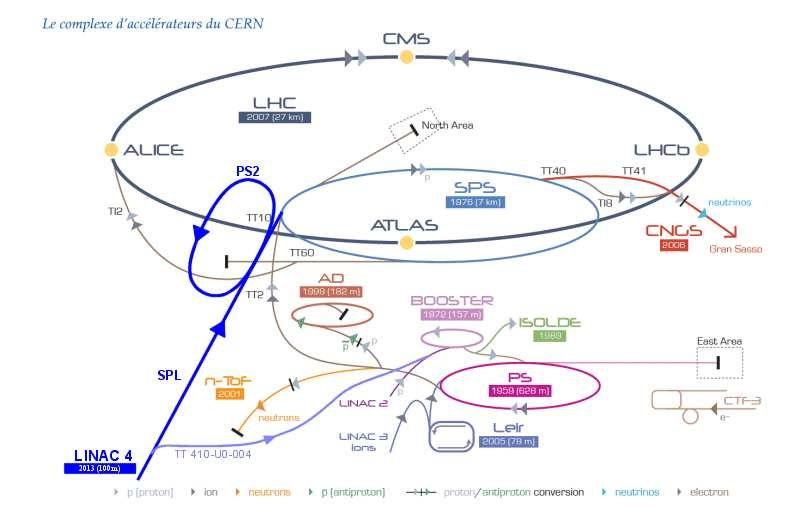
\includegraphics[scale = 0.4]{plots/lhc.png} 
  \caption{The LHC Accelerator Complex System.}
  \label{fig:LHC}
\end{figure}


\ \\This analysis is based on ATLAS (A Toroidal LHC ApparatuS) experimental data measurements.  ATLAS is one of the four LHC's detectors, being the largest machine ever built. It is a general-purpose particle physics, run by an international collaboration ~\cite{ATLAS}. 

\ \\The Standard Model is a theory that classifies the elementary particle (fermions and bosons) and describes three fundamental forces. It has 12 fermions that can be divided in two categories, quarks and leptons and they are the constituents of the matter. There are five bosons, the gluon which carry the strong force, photon responsible for electromagnetic force, W and Z bosons carrying the weak force. The most important boson is the Higgs, the responsible for the mass of all the elementary particles. 

\ \\Top quark is an interesting particle to study for several reasons: is the heaviest particle from the Standard Model (mt=173.3 GeV/c2) implies a high Yukawa coupling constant. Measuring the top-quark properties is the key to test the validity of the Standard Model.The . Another reason will be that decay very quickly (tau~10 -25 s). And if we find deviations in the top quark properties from the Standard Model predictions (e.g different cross-sections) implies the existence of new physics Beyond the Standard Model which is a very big purpose. Its evidence was discovered in March 1994 at CDF experiment at FermiLab in pp collisions at $s=\sqrt{1.8}$ TeV. Top quarks are produced in pairs by strong interactions by quark-antiquark annihilation 10\%, as gluon gluon fusion 90\%. The LHC has very high luminosity and the top quark are well understood. So because of this we can stay that the LHC is a top quark factory. 

\ \\At leading order the pair production of tt pairs is described by the following Feynman diagrams. We are interested about dileptonic channel. Even it is presented only in 2\% of the cases, it is advantageous because the background is very low comparing to others decay channel. The background comes in most of the cases from Z boson decay plus other jets.

\section{Neural Networks}

The goal of this project is to adapt a code example of machine learning unfolding (MLUnfolding) using toy data to use it for the jet energy reconstruction of ttbar e-mu analysis.

\ \\In this project one of the problems that we want to solve is the correction of detector smearing using Machine Learning. I have implemented this method using a sequential Neural Network. The unfolding correspond to an inversion of the migration matrix. Unfolding is the procedure to infer the truth data (what happened in reality in nature) from the reconstructed data (observed and measured in our experiment by our detector). The categorisation is a common problem for the modern Machine Learning methods. Possible methods could be boosted decision trees and Artificial Neural Networks. Neural Networks with various architectures can be tried for the unfolding problem.The unfolding involves several iterative steps of machine learning using a neural network training in TensorFlow via Keras, in Python. The NN takes as input the reconstructed values, and has as output the truth values.

\ \\The goal is to adapt this example to use real data coming from the jet pt distribution from the ttbar e-mu analysis. We use this .root flat tree~\cite{RootFile}.
This file contains both the reconstructed and truth jets, already matched. Meaning the i-th event from reco, corresponds to the i-th event from truth. Each jet collection collects jets already the jets ranked by pt. We take index 0 to consider the leading reco jet and the leading truth jet.

\ \\Given the leading jet pt as a continuous reco value, we want to find out in which jet pt bin (set by user, say 10 GeV or 20 GeV) does the truth jet falls. The input is a continuous value, but the output is a discrete value, that can take values from 0 to 49 if we consider 10 GeV bins from 0 to 500 GeV. Bin 0 contains jets with pt from 0 to 10 GeV. Jets with pt larger than 500 GeV have values set by hand to 499.999 GeV. It is equivalent to moving the overflow of a histogram bin to the last bin of the histogram. Given the output can take any value from 0 to 49, the problem we try to solve is a classification, and the possible labels are not only two (as in a simple signal to background classification, typically used in ATLAS), but a more complex one, with 50 labels. The NN will return the probability that for a given jet its pt falls in any of these bins. The total probability for all bins must be 1.0. This is ensured by the softmax activation function for the last layer of the NN. We then consider the bin with the largest probability as our choice by the NN. The predicted bin value can then be compared with the true bin value when making the plots of this project.

\ \\To optimize the NN performance, we take as input in fact not the jet pt, but the jet pt divided by the bin width. This is the jet pt bin as a real value. Making things more consistent with the output being the integer jet pt bin value for the truth.

\ \\ Neural Networks are an example of Machine Learning. In this way the computers learn a solution for a problem without being explicitly programmed. The two main classes of ML are supervised and unsupervised. 
In this project I used supervised ML. ......~\cite{AndrewNg}.

\ \\If we have the function Pi(y), a multidimensional highly non-linear, an efficient way to do this procedure is with an NN. This was inspired by the brain structure, which contains millions of neurone cells forming a network with electrochemical impulses passing between them. An artificial neural network formed by a number of interconnected artificial \emph{neurons}, or "nodes" respects this architecture. 

\ \\A network is formed by several ayers of nodes connected in series. Each node takes a weighted linear combination of the outputs from nodes of the previous layer, applies "activation function", then outputs the result do the next layer~\cite{AndrewNg}.

\ \\Using a "loss" function we can describe the difference between the predicted and real outputs, like the mean squared error between real and predicted. The weights associated with each node is modifies via an algorithm, and from here we can deduce that the loss function decreases and training increases.

\ \\We know from The \emph{Universal Approximation Theorem} that a neural network with one \emph{hidden layer} of nodes between input and output can in principle approximate any N-dimensional function to an arbitrary degree of accuracy, given a sufficiently large (though finite) number of nodes. 

\ \\In practice it is more suitable to use multiple hidden layers connected in series~\cite{AndrewNg}.

\section{The method}

My first step was to study a code example using some toy data in a JupyterNotebook~\cite{glazov}. At the beginning I ran the code on a cloud (Swan). 

\ \\The next step was to run it on \texttt{lxplus}. For this it was needed to run after \texttt{ssh}-ing to a \texttt{lxplus} machine a singularity command~\cite{Singularity} and then to my own laptop.

\ \\To train the neural network it was needed to use the Python library Keras~\cite{keras} and for backend TensorFlow~\cite{tensorflow}. My method of sampling was implemented using numpy~\cite{numpy}.






\begin{thebibliography}{11}

\bibitem{ATLAS} The ATLAS experiment, \url{https://atlas.cern}
\bibitem{RootFile} The ttbar e-mu ROOT file used {\tiny \texttt{\detokenize{/afs/cern.ch/user/l/lciucu/public/data/MLUnfolding/user.yili.18448069._000001.output.sync.root}}}
\bibitem{bendavid} Joshua Bendavid, \textit{Efficient Monte Carlo Integration Using Boosted Decision Trees and Generative Deep Neural Networks}, 2017
\bibitem{AndrewNg} Andrew Ng, \textit{Machine Learning. Coursera online course}, \url{URL https://www.coursera.org/learn/machine learning}
\bibitem{glazov} Alexander Glazov, \textit{Machine learning as an instrument for dana unfolding}, \textbf{arXiv}: 1712.01814v1, \url{http://inspirehep.net/record/1641082}
\bibitem{Singularity} The singularity command to run the ML environment, \\ {\tiny \texttt {\detokenize{singularity exec '/cvmfs/unpacked.cern.ch/registry.hub.docker.com/atlasml/ml-base:latest'bash}}}
\bibitem{keras} The keras machine learning library, \url{https://keras.io}
\bibitem{tensorflow} The TensorFlow machine learning library, \url{https:// www.tensforflow.org}
\bibitem{numpy} The Numerical Python library, \url{https://www.numpy.org}
\bibitem{topquark} \textit{Measurement of jet activity produced in top-quark events with an electron, a muon and two b-tagged jets in the final state in pp collision at s=13 TeV with the ATLAS detector}, \textbf{arXiv}: 1610.09978v2, \url{https://arxiv.org/pdf/1610.09978.pdf} 
\end{thebibliography}


\end{document}








\end{thebibliography}

\end{document}

%%%%%%%%%%%%%%%%%%%%%%%%%%%%%%%%%%%%%%%%%%
%%% example code - do not write below
%%%%%%%%%%%%%%%%%%%%%%%%%%%%%%%%%%%%%%%%%%%

\section{Introduction}

\subsection{Part 1...}

\paragraph{}
Here new paragraph starts...........
\paragraph{}
Here new paragraph starts...........
\paragraph{}
Here new paragraph starts........... \\

\newpage
		
Equation:
	
\begin{equation}
% \langle t_f q_f | t_i q_i \rangle = 
\lim_{\substack{\epsilon \rightarrow
0\\N\rightarrow \infty}} \int \dots \int \mbox{d}q_1 \dots \mbox{d}q_{N-1} \frac{\mbox{d}p_1}{2 \pi
\hbar} \dots \frac{\mbox{d}p_N}{2 \pi \hbar}\exp{\left( \frac{i}{\hbar} \sum_{j=1}^N
\left[ p_j (q_j - q_{j-1}) - \epsilon H\left(pj, \frac{q_j +
q_{j-1}}{2}\right)\right]\right)}
\end{equation}
\vspace{2cm}
\begin{align}
 \lim_{\substack{\epsilon \rightarrow 0 \\ N\rightarrow \infty}} \frac{i}{\hbar}
\epsilon \sum_{j=1}^N \left[p_j \left(\frac{q_j-q_{j-1}}{\epsilon}\right) - H\left( p_j,
\frac{q_j+q_{j-1}}{2}\right) \right] &= \frac{i}{\hbar} \int_{t_i}^{t_f} \mbox{d}t \left( p
\dot{q}-H(p,q)\right) \nonumber\\ 
&= \frac{i}{\hbar} \int_{t_i}^{t_f} \mbox{d}t L = \frac{i}{\hbar} S[q]
\end{align}
\vspace{2cm}

Table:

Consider the following mesons $\eta$, $\eta'$ and $K$ and their quark content\footnote{The mesons
are actually a superposition of these quarks.}:
\begin{center}
\begin{tabular}{c|c|c}
 meson & composition & approx. mass\\ \hline
$K^0$ &  $d\bar{s} \, , \,s\bar{d}$ &  $498 \mbox{MeV}$\\
$K^{+}$ & $u\bar{s}$ & $494 \mbox{MeV}$\\
$K^{-}$ & $s \bar{u}$ & $494 \mbox{MeV}$  \\
$\eta$ & $u \bar{u} \, , \, d \bar{d} \, , \, s \bar{s}$ & $548 \mbox{MeV}$ \\
$\eta'$ & $u \bar{u} \, , \, d \bar{d} \, , \, s \bar{s}$ & $958 \mbox{MeV}$ 
\end{tabular}
\end{center}


\newpage
	
Plot:

\begin{figure}[h]
\subfloat{\includegraphics[width=0.495\textwidth]{figure.jpg}}%\label{corr_and_rate-left}}
\subfloat{\includegraphics[width=0.495\textwidth]{figure.jpg}}%\label{corr_and_rate-right}}
\caption{Left: correlation for different $d$ ; Right: acceptance rate and
autocorrelation time for different $d$}
\label{corr_and_rate}
\end{figure}

\newpage
		
\subsection{Part 2...}

\paragraph{}
Here new paragraph starts...............................................................
...........................................................................................
..........................................................................................
...........................................................................................
\paragraph{}
Here new paragraph starts..........................................................................
...........................................................................................
..........................................................................................
...........................................................................................
\paragraph{}
Here new paragraph starts..........................................................................
...........................................................................................
..........................................................................................
........................................................................................... \\

\section{Conclusions}

Some text here..............................................................................

\section*{Acknowledgements}

Some text here..............................................................................

\begin{thebibliography}{11}
\bibitem{nagashima}
Yorikiyo Nagashima, Yoichiro Nambu, \textit{Elementary Particle Physics Volume 1: Quantum Field
Theory and Particles}, (WILEY-VCH, 2010)
\bibitem{FORTRAN}
W. H. Press, S. A. Teukolsky, W. T. Vetterling, B. P. Flannery, \textit{Numerical Recipes in
FORTRAN - The Art of Scientific Computing, 2nd Ed.} (Cambridge University Press, 1992)
\bibitem{buendia}
G. M. Buend\'{i}a, \textit{Comparison between the Langevin and the hybrid simulation techniques for
a free field theory}, J. Phys. A: Math. Gen. \textbf{22}, 5065-5072 (1989).
\bibitem{tapei}
T. Cheung and L. Li, \textit{Gauge theory of elementary particle physics}, (Oxford University
Press, 1984)
\bibitem{degrand}
T. DeGrand and C. DeTar, \textit{Lattice Methods for Quantum Chromodynamics}, (World Scientific,
2006)
\bibitem{topoactions}
W. Bietenholz, U. Gerber, M. Pepe, U.-J. Wiese, \textit{Topological Lattice Actions},
arXiv:1009.2146v4 [hep-lat] (20 Dec 2010)
\bibitem{openbcs}
M. L\"{u}scher, S. Schaefer, \textit{Lattice QCD without topology barriers},
CERN-PH-TH-2011-116, 26pp (May 2011)
\bibitem{Crecipes}
W. H. Press, S. A. Teukolsky, W. T. Vetterling, B. P. Flannery, \textit{Numerical Recipes in
C - The Art of Scientific Computing, 2nd Ed.} (Cambridge University Press, 1992)
\bibitem{andreas}
A. Nube, private communication.
\bibitem{wolff}
U. Wolff, \textit{Critical Slowing Down}, Nuclear Physics B (Proc. Suppl.) \textbf{17}, 93-102
(1990).
\end{thebibliography}
\end{document}
